\chapter{پیش‌زمینه}\markboth{پیش‌زمینه}{پیش‌زمینه}\label{chap:prerequisites}
\section{نظریه‌ی گراف}
در این بخش، نظریه‌ی گراف و نحوه‌ی نمادگذاری‌ را مرور خواهیم کرد. نمادگذاری ارائه شده در این بخش برای پیگیری بخش‌ها و فصل‌های بعدی مورد نیاز است.

\subsection{گراف، زیرگراف و یکریختی}
یک \خمیده{گراف}، یک دوتایی \گراف{G} است که در آن
$V = \{v_{1},v_{2},...,v_{n}\}$
یک مجموعه‌ی مرتب شامل $n$ گره‌ یا رأس است و
$E \subseteq V\times V$
مجموعه‌ی یال‌هاست. اندازه گراف برابر اندازه مجموعه \V تعریف می‌شود که در اینجا $n$ است.

گراف \گراف{G}، یک گراف \خمیده{بدون جهت} است اگر برای هر دو رأس
$v_{i},v_{j} \in V$، از اینکه
$\edge{v}{i}{j}{E}$
بتوان نتیجه گرفت که
$\edge{v}{j}{i}{E}$
؛ در غیر این صورت گراف \خمیده{جهت‌دار} است.

به هر یال به صورت \یال{i}{i}
یک \خمیده{دور} گفته می‌شود. بطور کلی بین دو رأس \Vi و \Vj در یک گراف، می‌تواند بیش از یک یال وجود داشته باشد. یک \خمیده{گراف ساده}، گرافی بدون دور است که بین هر دو رأس آن حداکثر یک یال وجود داشته باشد.

در این پایان‌نامه منظور از گراف، گراف ساده بدون جهت است؛ در غیر این صورت عبارت دقیق قید خواهد شد.

یک گراف ساده را می‌توان با \خمیده{ماتریس مجاورت} \A به اندازه $n\times n$نمایش داد. درایه $(i,j)$ از ماتریس \A برابر 1 است اگر یال \یال{i}{j} وجود داشته باشد. در غیر این صورت این درایه برابر صفر است. بدیهی است که ماتریس مجاورت یک گراف بدون جهت، متقارن است.

رئوس و/یا یال‌های یک گراف می‌توانند برچسب داشته باشند. یک گراف برچسب‌دار را با سه‌تایی $(V,E,l)$ نشان می‌دهیم که در آن $l: X \mapsto \Sigma$ تابعی است که یک برچسب از الفبای $\Sigma$ را به هر عضو مجموعه‌ی \X نسبت می‌دهد که \X می‌تواند بسته به اینکه رئوس یا یال‌ها و یا هر دو برچسب‌گذاری شده باشند به ترتیب برابر \V یا \E و یا $V\cup E$ باشد.

دو گراف \گراف{G} و
$\graph{G^{\prime}}{V^{\prime}}{E^{\prime}}$
\خمیده{یکریخت}\پانوشت{isomorph} (با نماد $G^{\prime} \simeq G$) هستند اگر تابع نگاشت دوسویی $f: V \rightarrow V^{\prime}$ (تابع یکریختی) وجود داشته باشد به طوری که
$(v_{i},v_{j}) \in E$
اگر و تنها اگر
$(f(v_{i}),f(v_{j})) \in E^{\prime}$
. اگر $G = G^{\prime}$ باشد آنگاه به $f$ تابع \خمیده{خودریختی}\پانوشت{automorph} می‌گویند. برای دو گراف برچسب‌دار $G(V,E,l)$ و $G^{\prime} = (V^{\prime},E^{\prime},l^{\prime})$ تابع یکریختی (همچنین خودریختی) باید رابطه 
$l(v_{i}) = l^{\prime}(f(v_{i}))$
 را به ازای هر $v_{i} \in V$ نیز ارضاء کند.
 
به یک تابع با آرگومان از نوع گراف، ناوردای گرافی
\پانوشت{\متنلاتین{graph invariant}} گفته می‌شود اگر به دو گراف یکریخت مقدار یکسانی نسبت دهد. مثلاً توابع تعداد رئوس و تعداد یال‌ها توابع ناوردای گرافی می‌باشند.

برای دو گراف \گراف{G} و $\graph{G^{\prime}}{V^{\prime}}{E^{\prime}}$، می‌گوییم $G^{\prime}$ یک \خمیده{زیرگراف} از $G$ است (با نماد $G^\prime \subseteq G$) اگر $V^\prime \subseteq V$ و $E^\prime \subseteq E$. اگر $G^\prime \subseteq G$ و $E^\prime$ شامل تمام یال‌های $(u,v) \in E$ باشد به طوری که $u,v \in V^\prime$، آنگاه می‌گوییم $G^\prime$ یک \خمیده{زیرگراف القایی} $G$ است و آن را با نماد $G^\prime \sqsubseteq G$ نشان می‌دهیم.

\subsection{همسایگی و درجه}
دو رأس \Vi و \Vj از گراف $G$ \خمیده{مجاور}\پانوشت{adjacent} و یا \خمیده{همسایه}\پانوشت{neighbour} هستند اگر $(v_i,v_j) \in E$. برای رأس $v$ همسایگی $\mN(v)$، مجموعه‌ی رئوسی است که در مجاورت آن قرار دارند؛ به عبارتی
$\mN(v) = \{v_i | (v,v_i) \in E\}$.
به تمام یال‌ها به فرم $(v,v_i) \in E$ \خمیده{یال‌های حادث}\پانوشت{incident} رأس $v$ گفته می‌شود.

\begin{figure}[ht]
\centering
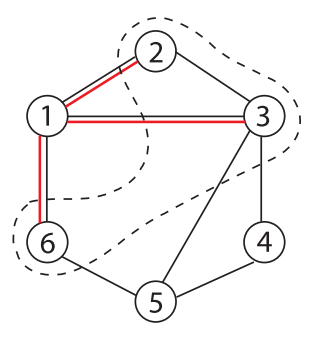
\includegraphics[scale=0.4]{./neighbours.png}
\caption{خط‌چین‌ رئوس همسایه‌ی رأس ۱ را نشان می‌دهد. یال‌هایی که با خطوط قرمز مشخص شده‌اند، یال‌های حادث هستند. درجه رأس ۱ برابر سه است.}
\label{fig:neighbours}
\end{figure}

درجه یک رأس مثل $v$ که با نماد $d(v)$ نشان داده می‌شود، تعداد یال‌های حادث با آن رأس است. برای گراف‌های ساده بدون جهت عدد اصلی\پانوشت{cardinality} مجموعه $\mN(v)$ با $d(v)$ برابر است.

\subsection{گشت، مسیر، دور، زیردرخت، الگوی زیردرختی}
یک \خمیده{گشت} در گراف، دنباله‌ای از رئوس است که دو رأس متوالی توسط یک یال به هم متصل شده‌باشند. یک \خمیده{مسیر}، گشتی است که تمام رئوس آن غیرتکراری باشند. به یک مسیر بسته \خمیده{دور} گفته می‌شود. گراف G \خمیده{همبند} است اگر بین هر دو رأس آن یک مسیر وجود داشته باشد. \خمیده{فاصله} بین دو رأس $v$ و $v^\prime$ در $G$ طول کوتاه‌ترین مسیر بین دو رأس $v$ و $v^\prime$ در $G$ است و اگر چنین مسیری وجود نداشته باشد، فاصله را برابر $\infty$ در نظر می‌گیریم.

% به زیرگراف همبند $G^\prime = (V^\prime,E\prime)$ از گراف \گراف{G} یک \خمیده{مؤلفه همبندی} گفته می‌شود
 
\begin{figure}[ht]
\centering
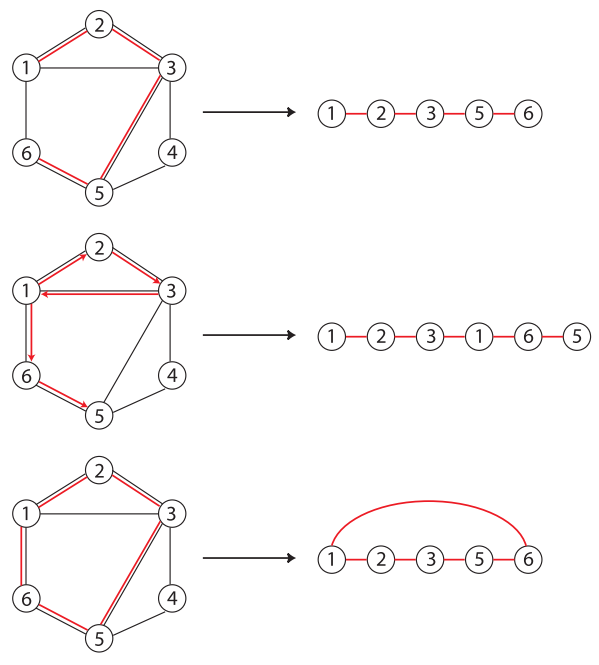
\includegraphics[scale=0.5]{./walk-path-cycle.png}
\caption{یک مسیر، یک گشت و یک دور.}
\label{fig:walk-path-cycle}
\end{figure}

یک زیردرخت (ریشه‌دار)، زیرگرافی بدون دور از یک گراف است که یک رأس از آن به عنوان ریشه در نظر گرفته می‌شود. ارتفاع این زیردرخت برابر است با طول طولانی‌ترین مسیر بین ریشه و سایر رئوس. همانطور که مفهوم گشت، توسعه‌ای از مفهوم مسیر است که در آن اجازه تکرار رئوس را داریم، مفهوم زیردرخت را می‌توان به مفهومی به اسم \خمیده{الگوی زیردرختی}\پانوشت{\متنلاتین{subtree pattern}} توسعه داد که در آن رئوس اجازه تکرار دارند (نام دیگری برای درخت-گشت‌\جستار{Bach_2008}.) رئوس تکراری به عنوان رئوس مجزا در این درخت در نظر گرفته می‌شوند به طوری که مفهوم درخت حفظ شود، یعنی در دور نداشته باشیم (شکل \ارجا{fig:subtree-pattern}).

\begin{figure}[ht]
\centering
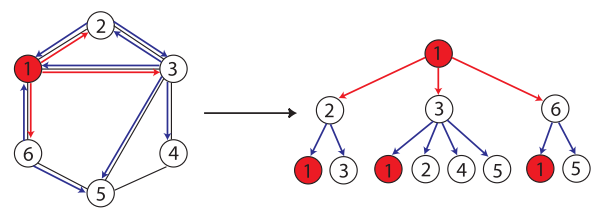
\includegraphics[scale=0.5]{./subtree-pattern.png}
\caption{یک الگوی زیردرختی به ارتفاع دو، ریشه گرفته از رأس ۱. به تکرار رئوس در الگوی زیردرختی توجه کنید.}
\label{fig:subtree-pattern}
\end{figure}

\section{مروری بر مقایسه‌ی گراف‌ها}\label{sec:graph_comparison}
مسئله اصلی مورد مطالعه در این پایان‌نامه، مقایسه‌ی گراف‌هاست. این مسئله در یک قالب رسمی به صورت زیر تعریف می‌شود.

\begin{definition}[مسئله‌ی مقایسه گراف‌ها]
اگر $\mG$ مجموعه‌ای از تمام گراف‌های ممکن باشد، مسئله‌ی مقایسه گراف‌ها، تعریف تابعی به شکل
\begin{equation*}
k:\mG \times \mG \mapsto \R,
\end{equation*}
است بطوری که $k(G,G^\prime)$ برای $G,G^\prime \in \mG$ نمایانگر شباهت $G$ و $G^\prime$ باشد.
\end{definition}
مقالات بسیاری در مبحث مقایسه‌ی دو گراف منتشر شده‌است که بطور کلی به دو دسته قابل تقسیم‌اند.

\subsection{روش‌های مبتنی بر یکریختی}
در این روش‌ها، از مفهوم یکریختی و یا مفاهیم مشابه نظیر زیرگراف یکریخت و بزرگترین زیرگراف مشترک استفاده می‌شود. بطور طبیعی ساده‌ترین راه اندازه‌گیری شباهت دو گراف این است که ببینیم آیا ساختار آن‌دو یکسان است یا خیر؛ که این مفهوم یکریختی است. این تعریف، سبب ایجاد تابعی می‌شود که دو مقدار دارد: اگر دو گراف یکریخت باشند، یک است و در غیر این صورت صفر است. اگرچه ایده‌ی این روش بسیار ملموس است، اما هیچ الگوریتم بهینه‌ای برای محاسبه مقدار این تابع وجود ندارد. مسئله بررسی یکریختی گراف، NP‌ است اما اینکه مسئله \متنلاتین{NP-complete} است یا الگوریتم حل در زمان خطی برای آن وجود دارد هنوز اثبات نشده‌است\جستار{Garey_1979}.

بررسی زیرگراف یکریخت همانند بررسی یکریختی گراف‌هاست، اما برای دو گراف با اندازه‌های مختلف تعریف می‌شود. برخلاف مسئله یکریختی، اثبات شده‌است که مسئله زیرگراف یکریخت جزء مسائل \متنلاتین{NP-complete} است\جستار{Garey_1979}.

یک معیار شباهت دیگر که محدودیت کمتری دارد، بر اساس اندازه بزرگترین زیرگراف مشترک بین دو گراف تعریف می‌شود. ولی مسئله پیدا کردن این زیرگراف \متنلاتین{NP-hard} است\جستار{Garey_1979}.

\subsection{روش‌های مبتنی بر فاصله ویرایش}
روش‌های مبتنی بر یکریختی، علاوه بر اینکه از لحاظ محاسباتی تقریباً غیرقابل استفاده هستند، گستره محدودی نیز دارند؛ از این لحاظ که دو گراف تحت بررسی یا باید دقیقاً یکسان باشند و یا زیرگراف‌های بزرگ مشترکی داشته باشند تا شبیه شمرده شوند. معیارهای انعطاف‌پذیرتری بر مبنای تطابق غیردقیق دو گراف وجود دارد. معیارهای مبتنی بر فاصله ویرایش در این دسته قرار دارند\جستار{Sanfeliu_1983}\جستار{Bunke_1983}\جستار{Messmer_1998}\جستار{Neuhaus_2005}. بر اساس این روش، دو گراف $G$ و $G^\prime$ شبیه هستند اگر یکی از آن‌ها را بتوان توسط تعداد کمی تغییر ساده مثل حذف و اضافه کردن رأس یا یال و یا تغییر برچسب‌گذاری (برای گراف‌های برچسب‌دار)، به دیگری تبدیل کرد. برای هر نوع تغییر هزینه‌‌ای متفاوت در نظر گرفته می‌شود و مقدار شباهت، برابر کمترین هزینه برای تبدیل $G$ به $G^\prime$ خواهد بود. متأسفانه پیدا کردن هزینه‌ی بهینه، مسئله ساده‌ای نیست.

بطور خلاصه، روش‌های مبتنی بر فاصله ویرایش، اگرچه معیارهای خوبی برای اندازه‌گیری شباهت ساختار گراف‌ها، و حتی رئوس و یال‌ها هستند، ولی در مراحل میانی اجرای الگوریتم، مسائل \متنلاتین{NP-complete} بوجود می‌آیند که در زمان خوبی قابل حل نیستند.

\section{مروری بر روش‌های نمایش گراف}\label{sec:graph_representation}
مسئله نمایش گراف به شکل زیر مطرح می‌شود.
\begin{definition}[مسئله نمایش گراف]
اگر $\mG$ مجموعه‌ای از تمام گراف‌های ممکن باشد، مسئله نمایش گراف‌، تعریف تابعی به شکل
\begin{equation*}
\phi:\mG \mapsto \R^p, p \in \N
\end{equation*}
است بطوری که برای هر $G \in \mG$،
 $\phi(G)$
  نمایانگر ساختار $G$ باشد.
\end{definition}

نمایش گراف و شباهت گراف دو مسئله نزدیک و مرتبط هستند: واضح است که اگر راه بهینه و کاملی برای خلاصه کردن ساختار یک گراف در قالب یک بردار ویژگی\پانوشت{\متنلاتین{feature vector}} وجود داشت، مقایسه گراف‌ها هم کار مشکلی نبود. در این بخش سه دسته‌ی مهم از روش‌های نمایش گراف را مختصر مرور می‌کنیم. همانطور که مشخص است هدف از این روش‌ها محاسبه برداری است که نمایانگر ساختار گراف باشد. هرکدام از این روش‌ها را می‌توان مستقیماً در تعریف یک تابع شباهت برای گراف‌ها بکار برد.

\subsection{واصف ساختاری}
خلاصه کردن ساختار یک گراف در قالب یک بردار برای اولین بار در شیمی محاسباتی صورت گرفت‌\جستار{Gasteiger_Engel_2003}. همانطور که در مقدمه ذکر شد، یک راه استاندارد برای نمایش مولکول، مدل کردن آن توسط گراف است که رئوس گراف، اتم‌ها و یال‌های گراف نمایانگر پیوندها هستند. یک \خمیده{واصف ساختاری}\پانوشت{\متنلاتین{topological descriptor}}(یا شاخص ساختاری\پانوشت{\متنلاتین{topological index}}) یک عدد یا بردار عددی است که ساختار گراف را توصیف می‌کند. این واصف‌های برداری، معمولاً  ناوردای گرافی هستند و در مسائل شیمی محاسباتی بجای ساختار مولکول‌ها بکار می‌روند.  از سال ۱۹۵۰، تعداد زیادی واصف ساختاری برای گراف‌ها تعریف شد (برای مطالعه کامل این واصف‌ها مراجعه شود به \جستار{Todeschini_2008}).

از مهمترین واصف‌های ساختاری، می‌توان به شاخص‌های وینر\پانوشت{Wiener}\جستار{Wiener_1947}، مرگان\پانوشت{Morgan}\جستار{Morgan_1965} و زاگرب\پانوشت{Zagreb}\جستار{Gutman_1972} اشاره کرد که در ادامه توضیح داده خواهند شد. شاخص وینر، مجموع طول تمام کوتاهترین مسیرهای یک گراف است.

\begin{definition}[شاخص وینر]
برای گراف \گراف{G}، شاخص وینر (عدد وینر) برابر است با
\begin{equation*}
W(G) = \sum_{v_i\in V}\sum_{v_j\in V} D_{ij}
\end{equation*}
که $D_{ij}$ طول کوتاهترین مسیر بین رئوس \Vi و \Vj است.
\end{definition}

شاخص مرگان، توسط رابطه بازگشتی زیر تعریف می‌شود.
\begin{definition}[شاخص مرگان]
برای گراف \گراف{G}، شاخص مرگان درجه $k$ برای هر رأس $v \in V$ برابر است با
\begin{equation*}
M_k(G,v) = 
\left\{
	\begin{array}{ll}
		\1  & \mbox{if } k = \0, \\
		{\sum_{v^\prime\in \mN(v)}M_{k-\1}(v^\prime)} & otherwise.
	\end{array}
\right.
\end{equation*}
در واقع، شاخص مرگان درجه $k$ برای رأس $v$ برابر است با تعداد گشت‌هایی به طول $k$ با شروع از رأس $v$ در گراف $G$.
\end{definition}

\begin{definition}[شاخص زاگرب]
برای گراف \گراف{G}، شاخص‌های اول و دوم زاگرب به ترتیب به صورت
\begin{equation*}
Z_\1(G) = \sum_{v\in V}(d(v))^\2
\end{equation*}
و
\begin{equation*}
Z_\2(G) = \sum_{(v,v^\prime)\in E}d(v)d(v^\prime)
\end{equation*}
تعریف می‌شوند که $d(v)$ درجه رأس $v$ است.
\end{definition}

هر سه این تعاریف، ناوردای گرافی هستند: یعنی اگر دو گراف $G$ و $G^\prime$ یکریخت باشند، مقدار واصف ساختاری آن‌ها تحت تعاریف بالا یکسان خواهد بود. ولی عکس این حالت صادق نیست. واضح است که تعریف واصف گرافی که بتواند حالت عکس را نیز تأمین کند، معادل حل مسئله یکریختی است که برای آن الگوریتم خطی پیدا نشده‌است.  باید توجه داشت که ممکن است یکی از واصف‌های گرافی در یک مسئله، پاسخ‌های بهتری بدهد ولی در مسئله دیگر واصف دیگری بهترین پاسخ را داشته باشد. انتخاب بهترین واصف گرافی از بین تعداد زیادی از آن‌ها برای یک مسئله‌ی خاص، بسیار سخت است.

\subsection{استخراج الگو‌های متواتر}
استخراج الگوهای متواتر\پانوشت{\متنلاتین{frequent pattern mining}} یکی از زیرشاخه‌های داده‌کاوی است. اگر زیرگراف‌ها را به عنوان الگو در نظر بگیریم، آنگاه استخراج زیرگراف‌های متواتر، روشی برای یافتن زیرگراف‌هایی است که در یک مجموعه گراف، بیشترین تکرار را دارند.

نمایش گراف بوسیله استخراج زیرگراف‌های متواتر، به این شکل انجام می‌شود: برای هر $G \in \mG$، و برای هر زیرگراف انتخابی $g_i$، تعداد تکرار آن زیرگراف در $G$ ثبت می‌شود. در پایان برای هر $G$ برداری به شکل
\begin{equation*}
(c_\1(G),...,c_p(G))
\end{equation*}
خواهیم داشت که در آن $c_i(G)$ برابر تعداد تکرار زیرگراف $g_i$ در $G$ است و $p$ تعداد این زیرگراف‌هاست.

بسیاری از الگوریتم‌های استخراج الگوهای متواتر بر مبنای خصوصیتی به نام \خمیده{انتاج}\پانوشت{Apriori}\جستار{Agrawal_1994} عمل می‌کنند. این مفهوم بیان می‌کند که اگر یک مجموعه $S$ در گردایه‌ای از مجموعه‌ها، متواتر باشد، آنگاه هر زیرمجموعه از $S$ هم متواتر خواهد بود. این مشاهده به سادگی قابل تعمیم به گراف‌هاست: اگر گراف $H$ در مجموعه‌ای از گراف‌ها مکرراً دیده شود، آنگاه هر زیرگرافی از $H$ هم حداقل به اندازه $H$ دیده خواهد شد، لذا این زیرگراف‌ها نیز متواتر خواهند بود. الگوریتم AGM \جستار{Inokuchi_2000} یک مثال خوب از الگوریتم‌های مبتنی بر انتاج برای استخراج زیرگراف‌های متواتر است.

روش‌های رشد-الگو\پانوشت{pattern-growth}\جستار{Han_2000}، دیگر گروه مهم در الگوریتم‌های استخراج زیرگراف‌های متواتر هستند. این الگوریتم‌ها، کار را با الگوهای کوچک آغاز می‌کنند و در مراحل بعد، آنها را گسترش می‌دهند تا حدی که الگوهای بدست آمده دیگر متواتر نباشند. مهمترین مثال‌ها از این خانواده، الگوریتم gspan \جستار{Yan_2002} و Gaston \جستار{Nijssen_2005} هستند. در gspan، یک ترتیب الفبایی برای گراف‌های برچسب‌دار بر حسب الگوریتم جستجوی عمق-اول (DFS) تعریف شده و هر گراف به یک برچسب متعارف یکتا (با نام \خمیده{کوتاهترین کد DFS}) نگاشت می‌شود. فضای جستجو در gspan به صورت درختی از کدهای DFS در نظر گرفته می‌شود که هر برگ در این درخت توسط روشی برای گسترش الگوها (با نام \خمیده{راست‌ترین بسط}\پانوشت{\متنلاتین{rightmost extension}}) بدست می‌آید. بدین طریق، gspan در حین جستجو برای زیرگراف‌های متواتر، از تست دوباره یک الگو و یا گسترش یک الگو که قبلاً دیده‌است جلوگیری می‌کند.

روش‌های جستجوی زیرگراف‌های متواتر، در مسائل یادگیری روی گراف‌های کوچک خوب عمل می‌کنند. مشکل بزرگ این روش‌ها این است که فضای جستجو در رابطه با اندازه‌ی گراف، رشد نمایی دارد و با وجود الگوریتم‌های هوشمندانه (همچون استفاده از روش‌های شاخه و حد\پانوشت{\متنلاتین{branch and bound}})، در بدترین حالت باید تمام زیرگراف‌های یک گراف را بشمارند که اینکار برای گراف‌های بزرگتر از بیست رأس عملاً غیرقابل انجام است.

\section{مروری بر گراف کرنل‌ها}\label{sec:graph-kernels-review}
همانطور که در بخش‌های \ارجا{sec:graph_comparison} و \ارجا{sec:graph_representation} دیدیم، روش‌های سنتی مقایسه و نمایش دو گراف از مشکلاتی نظیر زمان اجرای نمایی و عدم توان در خلاصه‌سازی بهینه ساختار گراف رنج می‌برند و یا پارامتربندی و استفاده از آن‌ها در کاربردهای همه منظوره، دشوار است. گراف کرنل‌ها که اخیراً به عنوان ابزار یادگیری روی داده‌های ساختاری، برای خود جایی باز کرده‌اند، سعی در رفع این مشکلات دارند. این ابزارها می‌توانند همزمان به خلاصه‌سازی و مقایسه گراف‌ها بپردازند، ولی با محدود کردن خود به زیرساختارهایی از گراف که اجازه محاسبه مقدار کرنل در زمان خطی را می‌دهد، از بروز مشکلات پیشین جلوگیری می‌کنند. گراف کرنل‌ها، فاصله بین داده‌های گرافی و طیف وسیعی از الگوریتم‌های یادگیری ماشین با نام \خمیده{روش‌های کرنل}\جستار{Scholkopf_2002} را پر می‌کنند. الگوریتم‌های \متنلاتین{kernel PCA} و \متنلاتین{SVM} از این دسته‌اند.

قبل از مرور گراف کرنل‌ها، توابع کرنل در یادگیری ماشین را مختصراً توضیح می‌دهیم. برای شرح جامع به کتاب «یادگیری به وسیله کرنل‌ها»\جستار{Scholkopf_2002} مراجعه شود.

\subsection{کرنل‌ها در یادگیری ماشین}
بطور ساده، کرنل (مثبت معین) تابعی است که شباهت دو شیء را می‌سنجد. در این بخش ابتدا به معرفی کرنل می‌پردازیم و سپس یک مثال از کاربرد تابع کرنل را در قالب دسته‌بندی دودویی\پانوشت{\متنلاتین{binary classification}} خواهیم دید.

\subsubsection{کرنل‌های مثبت معین}\label{sec:positive-semidefinite-kernels}
در زیر تعریف کرنل‌های نیمه معین مثبت که از کتاب \جستار{Scholkopf_2004} آورده شده را می‌آوریم.
\begin{definition}[کرنل‌ نیمه معین مثبت]
اگر $\mX$ یک مجموعه ناتهی باشد، تابع $k: \mX \times \mX \mapsto \R$ یک تابع کرنل نیمه معین مثبت است اگر و تنها اگر متقارن باشد، یعنی برای هر $x,x^\prime \in \mX$ داشته باشیم
$k(x,x^\prime) = k(x^\prime,x)$، و نیمه معین مثبت باشد، 
یعنی برای هر $N \in \N$، هر انتخاب از اشیاء $x_\1,...,x_N \in \mX$ و هر انتخاب از اعداد حقیقی $c_\1,...,c_N \in \R$ داشته باشیم:

\begin{equation*}
\sum_{i=\1}^{N}\sum_{j=\1}^{N}c_ic_jk(x_i,x_j) \geq 0
\end{equation*}
\end{definition}

در یادگیری ماشین، به کرنل‌های نیمه معین مثبت معمولاً کرنل‌های مثبت معین یا خلاصه‌تر، کرنل گفته می‌شود. در ادامه این پایان‌نامه از واژه‌ی کرنل برای اشاره به این تعریف استفاده می‌کنیم.

چرا کرنل‌ها در یادگیری ماشین مورد توجه قرار گرفته‌اند؟ پاسخ این است که این توابع، امکان محاسبه ضرب‌داخلی در فضای با بعد بالا را در زمان بهینه فراهم می‌آورند که اینکار برای بسیاری از تکنیک‌های یادگیری ماشین ضروری است. شرح این پاسخ در ادامه آورده شده است.

خصوصیت اصلی کرنل‌ها که توجیه کننده ارتباط آن‌ها با ضرب داخلی است، این است که: برای هر کرنل نیمه معین مثبت $k: \mX \times \mX \mapsto \R$ یک فضای هیلبرت  بازتولیدِ کرنل \پانوشت{\متنلاتین{reproducing kernel Hilbert space}}
(RKHS) $\mH$ و یک تابع نگاشت $\phi: \mX \mapsto \mH$ وجود دارد بطوری که
به ازای هر $x,x^\prime \in \mX$،
$k(x,x^\prime)$
 برابر ضرب داخلی 
 $\phi(x)$ 
 و $\phi(x^\prime)$ است:
\begin{equation*}
k(x,x^\prime) = \langle\phi(x),\phi(x^\prime)\rangle.
\end{equation*}
عکس این خاصیت هم درست است: اگر $\mX$ یک مجموعه ناتهی باشد، $\mH$ یک فضای هیلبرت بازتولید کرنل باشد و $\phi: \mX \mapsto \mH$ تابع نگاشت باشد، آنگاه هر تابع $k: \mX\times \mX \mapsto \R$ که به وسیله $k(x,x^\prime) = \langle\phi(x),\phi(x^\prime)\rangle$ مشخص شده باشد، یک تابع کرنل نیمه معین مثبت است. در یادگیری ماشین، به $\mH$ فضای ویژگی\پانوشت{\متنلاتین{feature space}}،
به $\phi$ تابع نگاشت ویژگی\پانوشت{\متنلاتین{feature map}} و
به $\phi(x)$ نمایش ویژگی
\پانوشت{\متنلاتین{feature representation}}
$x$ می‌گویند.

در حقیقت، تعریف تابع نگاشت ویژگی، راه مستقیم تعریف یک کرنل است. به عنوان مثال فرض کنید که به ازای یک $p$، 
$\mX = \R^p$، $\mX = \mH$ و $\phi$ را برابر تابع همانی در نظر بگیریم، آنگاه تابع
\begin{equation*}
k(x,x^\prime) = \langle\phi(x),\phi(x^\prime)\rangle = \langle{x,x^\prime}\rangle
\end{equation*}
که یک ضرب داخلی ساده است، کرنل معتبری است.

این مثال در واقع راهی را برای طراحی هر تابع کرنل دلخواه، پیش رو می‌گذارد:
\begin{enumerate}
\فقره $\mH$ را انتخاب کنید،
\فقره تابع نگاشت $\phi$ را انتخاب کنید،
\فقره قرار دهید: $k(x,x^\prime) = \langle\phi(x),\phi(x^\prime)\rangle $.
\end{enumerate}

هرچند این روند برای تعریف کرنل، کاملاً درست است، ولی هیچ کمکی به محاسبه $\langle\phi(x),\phi(x^\prime)\rangle$ نمی‌کند: برای محاسبه $k(x,x^\prime)$، هنوز لازم است که ضرب و جمع در فضای $\mH$ صورت پذیرد که زمان اجرای آن متناسب با بُعد فضای $\mH$ خواهد بود. اما نکته جالب اینجاست که برای بعضی از کرنل‌ها، می‌توان بدون محاسبه در فضای $\mH$، مقدار $k(x,x^\prime)$ را بدست آورد. این ویژگی است که موجب اقبال روش‌های مبتنی بر کرنل در یادگیری ماشین شده‌است. به کمک این ویژگی، می‌توان نمایش داده در فضای $\mH$ را با بُعد بسیار بالا و حتی بی‌نهایت در نظر گرفت. برای روشن شدن موضوع، دو کرنل معروف \خمیده{چندجمله‌ای}\پانوشت{polynomial} و \خمیده{تابع شعاع محور گاوسی}(RBF)\پانوشت{\متنلاتین{gaussian radial basis function}} را در فضای $\R^p\times \R^p$ بررسی می‌کنیم.

\paragraph{کرنل چند جمله‌ای}
این کرنل به وسیله تابع زیر تعریف می‌شود:
\begin{equation*}
k(x,x^\prime) = (\langle{x,x^\prime}\rangle + c)^d
\end{equation*}
که در آن $d \in N$ و $c \geq \0 $ پارامتر هستند. می‌توان نشان داد که بُعد فضای ویژگی برای $k$ برابر تعداد تک جمله‌ای ها با درجه $d$ و یا کمتر در $p$ متغیر است، که برابر است با $p+d\choose d$. فرض کنید که $ p = 100 $ و $ d = 4 $: محاسبه $k(x,x^\prime)$ در ۲۰۲ عمل (۱۰۲ ضرب و ۱۰۰ جمع) انجام خواهد شد، درحالی که محاسبه مقدار تابع توسط نمایش ویژگی $\phi(x)$ و $ \phi(x^\prime) $، 
$2{104\choose 4} - 1 = 2\times 4598126−1 = 91962522$ عمل جمع و ضرب نیاز خواهد داشت. بنابراین کرنل چندجمله‌ای این امکان را فراهم می‌آورد که ضرب‌داخلی در فضای 
$\R^{4598126}$  را بجای حدود ۹ میلیون عمل، طی ۲۰۲ عمل ضرب و جمع انجام دهیم.
اینکار برای درجات بالاتر $d$ و مقادیر بزرگتر $p$ بهبود چشمگیری در زمان اجرای محاسبه است.

\paragraph{کرنل شعاع محور گاوسی}
 این کرنل به شکل 
\begin{equation}\label{eq:gaussian-kernel}
k(x,x^\prime) = exp(-\dfrac{\|x - x^\prime\|^2}{2\sigma^2})
\end{equation}
تعریف می‌شود که در آن $\sigma > 0$. ویژگی این کرنل آن است که فضای \متنلاتین{RKHS} متناظر با آن بی‌نهایت-بُعدی است. نمایشِ داده در این فضا غیر ممکن است، اما با کمک تابع کرنل می‌توان مقدار ضرب داخلی در این فضا را بدست آورد.

چطور بدون انتخاب صریح فضای $\mH$ و تابع $\phi$ یک کرنل نیمه معین مثبت تعریف کنیم؟ یک راه ساده، استفاده از خاصیت بسته بودن مجموعه کرنل‌های نیمه معین مثبت نسبت به بعضی از عمل‌هاست که به این وسیله می‌توان کرنل‌های جدیدی تعریف کرد\جستار{Scholkopf_2002}. در زیر به بعضی از این خواص اشاره می‌کنیم:

\begin{itemize}
\فقره اگر $k_1$ و $k_2$ کرنل و 
$\alpha_1,\alpha_2 \geq 0$ باشند
 آنگاه $\alpha_1k_1 + \alpha_2k_2$ یک کرنل است.
\فقره اگر $k_1,k_2,...$ کرنل باشند و 
$k(x,x^\prime) = \lim_{n \to \infty}k_n(x,x^\prime)$
برای تمام $x$ و $x^\prime$ وجود داشته باشد، آنگاه $k$ کرنل است.
\فقره اگر $k_1$ و $k_2$ کرنل باشند آنگاه $k_1k_2$ که به صورت 
$k_1k_2(x,x^\prime) = k_1(x,x^\prime)k_2(x,x^\prime)$ تعریف می‌شود، هم کرنل است .
\end{itemize}

کرنل‌ها علاوه بر اینکه امکان محاسبه‌ی ضرب داخلی در فضای با بعد بالا را فراهم می‌آورند، این قدرت را دارند که از داده‌های غیربرداری هم استفاده کنند. اگر برای هر شیء دلخواه، تابع متقارنی به عنوان مقیاس شباهت آن اشیاء تعریف کنیم، و اثبات کنیم که این تابع، نیمه معین مثبت است آنگاه بطور خودکار نمایشِ برداریِ داده در فضای ویژگی را در درست داریم و از آن برای محاسبه‌ی ضرب داخلی استفاده می‌کنیم.

رابطه‌ی بین کرنل‌ها و اندازه‌گیری شباهت جالب توجه است: در بین محققان رشته یادگیری ماشین، ضرب‌داخلی به عنوان معیاری از شباهت در نظر گرفته می‌شود. برای روشن شدن موضوع ابتدا رابطه‌ی فاصله و شباهت را در نظر بگیرید. اگر نوعی از فاصله (مثلاً فاصله اقلیدسی) بین دو شیء کم باشد، آنگاه این دو شیء طبق آن فاصله شبیه هم در نظر گرفته می‌شوند. می‌توان نشان داد که برای هر کرنل $k$ روی هر $\mX$ رابطه
\begin{equation*}
k(x,x^\prime) = \dfrac{\|\phi(x)\|^2 + \|\phi(x^\prime)\|^2 - \|\phi(x) - \phi(x^\prime)\|^2}{2}
\end{equation*}
که در آن $\|z\| = \langle{z,z}\rangle$، برقرار است. همانطور که در فصل یک از \جستار{Scholkopf_2004} توضیح داده شده‌است، $k(x,x^\prime)$ مقدار شباهت بین $x$ و $x^\prime$ را در قالب عکس مجذور فاصله بین $\phi(x)$ و $\phi(x^\prime)$ در فضای ویژگی، تا جمله 
$\|\phi(x)\|^2$ و
$\|\phi(x^\prime)\|^2$
 اندازه می‌گیرد. اگر در این فضا تمام نقاط، طول یکسانی داشته باشند (برای هر $x \in \mX$ مقدار $\|\phi(x)\|^2$ عددی ثابت باشد)، آنگاه کرنل یک تابع کاهشی از فاصله در فضای ویژگی است.

به عنوان جمع‌بندی این بخش باید گفت از آنجا که کرنل‌ها حاصل ضرب‌داخلی هستند، می‌توان به آنها بعنوان مقیاس شباهت نگاه کرد. و از آنجا که برای هر کرنل، یک تابع نگاشت ویژگی وجود دارد، می‌توان آنها را ابزاری برای نمایش گراف در نظر گرفت. برای بعضی کرنل‌ها، تعریف دقیق نحوه نمایش گراف امکان‌پذیر نیست. اما براساس آنچه توضیح داده شد، محاسبه ضرب داخلی در فضای ویژگی امکان‌پذیر است. علاوه بر این، یک امتیاز کرنل این است که برای انواع داده قابل تعریف هستند.

\subsubsection{دسته‌بندی دودویی با استفاده از ماشین‌های بردار پشتیبان}
دسته‌بندی دودویی یکی از مسائل بنیادی در یادگیری ماشین است و به این صورت مطرح می‌شود که با در اختیار داشتن دو دسته شیء، رابطه‌ای تعریف کنید که مشخص کند یک شیء‌ جدید به کدام دسته متعلق است. تعریف رسمی مسئله به این صورت است. یک مجموعه از دوتایی ها به شکل
\begin{equation*}
(x_1,y_1),...,(x_N,y_N) \in \mX \times \mY
\end{equation*}
در اختیار داریم که $\mX$ مجموعه‌ای از اشیاء (نمونه‌ها یا داده نقاط) و $\mY = \left\lbrace-1,+1 \right\rbrace$ است. $\mX$ می‌تواند مجموعه‌ای از هر چیز باشد: مجموعه‌ی موجودات زنده، شرایط آب و هوایی، ساختارهای پروتئینی و یا بردارهای به طول $p$. برای یک $x_i \in \mX$، $y_i$ مشخص کننده دسته‌ای است که $x_i$ به آن تعلق دارد و به آنها برچسب دسته یا فقط برچسب گفته می‌شود. هدف آن است که تابع $f: \mX \mapsto \mY$ را طوری تعریف کنیم که بتواند به نمونه‌های دیده نشده، برچسب درستی تخصیص دهد.

الگوریتم \خمیده{ماشین بردار پشتیبان}\پانوشت{\متنلاتین{Support Vector Machine}} یا به اختصار SVM برای یافتن تابع $f$، اولین بار در دهه ۱۹۶۰ توسط وپنیک\پانوشت{Vapnik} و لرنر\پانوشت{Lerner} طراحی شد\جستار{Vapnik_1963} و توسط بوزر\پانوشت{Boser} و دیگران\جستار{Boser_1992}، کورتز\پانوشت{Cortes} و وپنیک\جستار{Cortes_1995} به شکل امروزی آن فرمول‌بندی گشت. این الگوریتم به دلیل داشتن پایه‌ی قوی ریاضی و استفاده از خوش رفتارترین مسئله‌ی بهینه سازی‌ یعنی بهینه‌سازی‌ محدب\پانوشت{\متنلاتین{Convex Optimization}}، مورد توجه قرار گرفت. در ادامه، مبانی این الگوریتم را مرور خواهیم کرد. برای شرح مفصل‌تر به \جستار{Steinwart_2008} مراجعه شود.

مسئله دسته‌بندی دودوییِ SVM، روی داده ورودی به شکل 
$(\mx_1,y_1),...,(\mx_N,y_N) \in \mH\times\left\lbrace -1,+1 \right\rbrace$
 فرمول‌بندی می‌شود که در آن $\mH$ فضای هیلبرت بازتولید کرنل است. تفاوت این تعریف با تعریف قبلی در آن است که نمونه‌های $\mx_1,...,\mx_N$ برخلاف قبل نه یک مجموعه دلخواه بلکه متعلق به یک RKHS هستند. بدون از دست رفتن کلیت مسئله می‌توانیم هر $\mx_i$ را نمایش برداری شیء $x_i$ در نظر بگیریم. حتی می‌توان $\mX$ را یک RKHS در نظر گرفت، چون تنها شرط روی $\mX$ تهی نبودن است. هر عنصر از $\mx_i$ به عنوان ویژگی\پانوشت{feature} شناخته می‌شود. هدف SVM یافتن اَبَرصفحه‌ای است که نمونه‌های دو دسته را با بیشترین حاشیه\پانوشت{margin} از یکدیگر جدا کند، یعنی فاصله‌ی ابرصفحه از نقاط در بیشترین حالت ممکن باشد (شکل \ارجا{fig:svm-margin} را ببینید). اینکار معادل حل مسئله بهینه‌سازی زیر است.
 
\begin{figure}[ht]
\centering
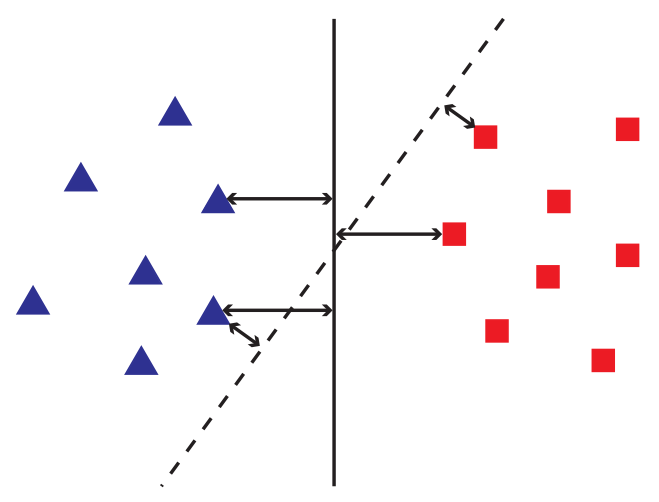
\includegraphics[scale=0.3]{./svm-margin.png}
\caption{مثلث‌ها و مربع‌ها نشان دهنده دو دسته از اشیاء در صفحه $\R^2$ هستند. خط‌چین و خط صاف دو ابرصفحه‌ی جدا کننده را نشان می‌دهند. ابرصفحه‌ی ‌صاف، نسبت به ابرصفحه‌ی ‌خط‌چین، دارای حاشیه‌ی ‌بیشتری از نقطه‌داده‌هاست. نقطه‌داده‌هایی که فاصله‌ی آن‌ها از ابرصفحه برابر انداز‌ه‌ی حاشیه است، بردارهای پشتیبان خوانده می‌شوند.}
\label{fig:svm-margin}
\end{figure} 
 
\begin{equation}\label{eq:svm-normal-form}
\begin{aligned}
& \underset{w \in \mH, b \in \R}{\text{minimize}} & & \dfrac{1}{2} \|w\|^2 \\
& \text{\lr{subject to}} & & y_i(\langle \mx_i,w \rangle + b) \geq 1 \quad\text{\lr{for all}}\quad i = 1, \ldots ,N.
\end{aligned}
\end{equation}
مسئله \ارجا{eq:svm-normal-form} معمولاً در فرم دوگانی لاگرانژ حل می‌شود:
\begin{equation}\label{eq:svm-dual-form}
\begin{aligned}
& \underset{\alpha \in \R^N}{\text{minimize}} & & W(\alpha)=\sum_{i=1}^{N}\alpha_i - \dfrac{1}{2} \sum_{i,j=1}{N} \alpha_i \alpha_j y_i y_j \langle \mx_i,\mx_j \rangle \\
& \text{\lr{subject to}} & & \alpha_i \geq 0 \quad\text{\lr{for all}}\quad i = 1, \ldots ,N, \\
& \text{\lr{and}} & & \sum_{i=1}^{N} \alpha_i y_i = 0.
\end{aligned}
\end{equation}
اگر داده نقاط مثبت و منفی توسط یک ابرصفحه، جدایی‌پذیر یا به اصطلاح \خمیده{خطی جدایی‌پذیر} باشند، حاصل حل مسئله \ارجا{eq:svm-normal-form}، ابرصفحه‌ی بهینه است (مثل شکل \ارجا{fig:svm-margin}). ولی داده نقاط همیشه خطی جدایی‌پذیر نیستند. نوعی از SVM ها با نام SVM‌ های \خمیده{حاشیه-ملایم}\پانوشت{\متنلاتین{soft-margin}} وجود دارند که می‌توانند روی داده نقاط تقریبا خطی جدایی‌پذیر (شکل \ارجا{fig:almost-linearly-separable}) کار کنند\جستار{Cortes_1995}. به این نوع از SVM ها، C-SVM می‌گویند. فرم اولیه و دوگانی C-SVM ها در ادامه آمده است.

\begin{figure}[ht]
\centering
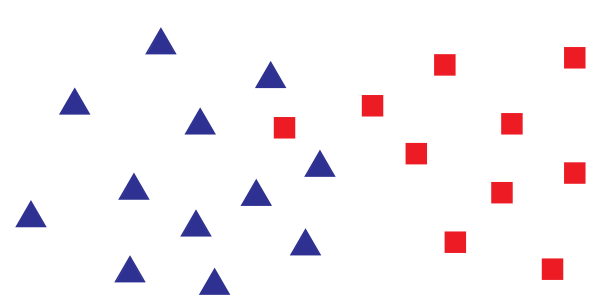
\includegraphics[scale=0.3]{./almost-linearly-separable.png}
\caption{دو دسته‌ی \خمیده{تقریباً} خطی جدایی پذیر.}
\label{fig:almost-linearly-separable}
\end{figure}

\begin{equation}\label{eq:c-svm-normal-form}
\begin{aligned}
& \underset{w \in \mH, b \in \R}{\text{minimize}} & & \dfrac{1}{2} \|w\|^2 + \dfrac{C}{N} \sum_{i=1}^{N} \xi_i \\
& \text{\lr{subject to}} & & y_i(\langle \mx_i,w \rangle + b) \geq 1 - \xi_i \quad\text{\lr{for all}}\quad i = 1, \ldots ,N, \\
& \text{\lr{and}} & & \xi_i \geq 0\quad\text{\lr{for all}}\quad i = 1, \ldots ,N.
\end{aligned}
\end{equation}
به $\xi_i$ ها متغیرهای کمکی\پانوشت{slack} گفته می‌شود. این متغیرها میزان نقض قید $y_i(\langle \mx_i,w \rangle + b) \geq 1$ توسط داده نقطه $i$ را اندازه می‌گیرند. در واقع این متغیرها اجازه می‌دهند داده نقاط تا اندازه‌ای غلط دسته‌بندی شوند. پارامتر $C$ برقرار کننده‌ی تعادل بین رساندن حاشیه به حداکثر و رساندن تعداد نقاطی که در حاشیه و یا در دسته غلط قرار گرفته‌اند، به حداقل است.
\begin{equation}\label{eq:c-svm-dual-form}
\begin{aligned}
& \underset{\alpha \in \R^N}{\text{minimize}} & & W(\alpha)=\sum_{i=1}^{N}\alpha_i - \dfrac{1}{2} \sum_{i,j=1}{N} \alpha_i \alpha_j y_i y_j \langle \mx_i,\mx_j \rangle \\
& \text{\lr{subject to}} & & 0 \leq \alpha_i \leq \dfrac{C}{N} \quad\text{\lr{for all}}\quad i = 1, \ldots ,N, \\
& \text{\lr{and}} & & \sum_{i=1}^{N} \alpha_i y_i = 0.
\end{aligned}
\end{equation}
C-SVM ها مسئله‌ی پیدا کردن ابرصفحه‌ی ‌بهینه برای جداسازی دو دسته را طوری حل می‌کنند که در آن به تعداد کمی از داده نقاط اجازه داده می‌شود که غلط دسته‌بندی شوند. ولی برخی از مسائل هستند که نمی‌توان با تعداد کمی اشتباه، داده ها را با یک ابرصفحه از هم جدا کرد، هر ابرصفحه‌ای که انتخاب کنیم تعداد زیادی از نقاط اشتباه دسته‌بندی می‌شوند (شکل \ارجا{fig:non-linearly-separable-data} را ببینید). در این حالت شاید بتوان نمایش داده نقاط را طوری بازتعریف کرد که خطی جدایی‌پذیر بشوند.
همانطور که در شکل \ارجا{fig:non-linearly-separable-data}  نشان داده شده‌است، حتی در مواردی که داده‌ها به شدت غیر خطی هستند، می‌توان از الگوریتم دسته‌بندی خطی  SVM استفاده‌کرد و از قابلیت‌های آن بهره برد. تنها شرطی که دارد آن است که بتوانیم داده نقاط را در یک فضای دیگر طوری بازنشانی کنیم که خطی جدایی‌پذیر بشوند. اولین چیزی که به ذهن خطور می‌کند استفاده از فضاهای با بعد بالاتر RKHS است.

\begin{figure}[ht]
\centering
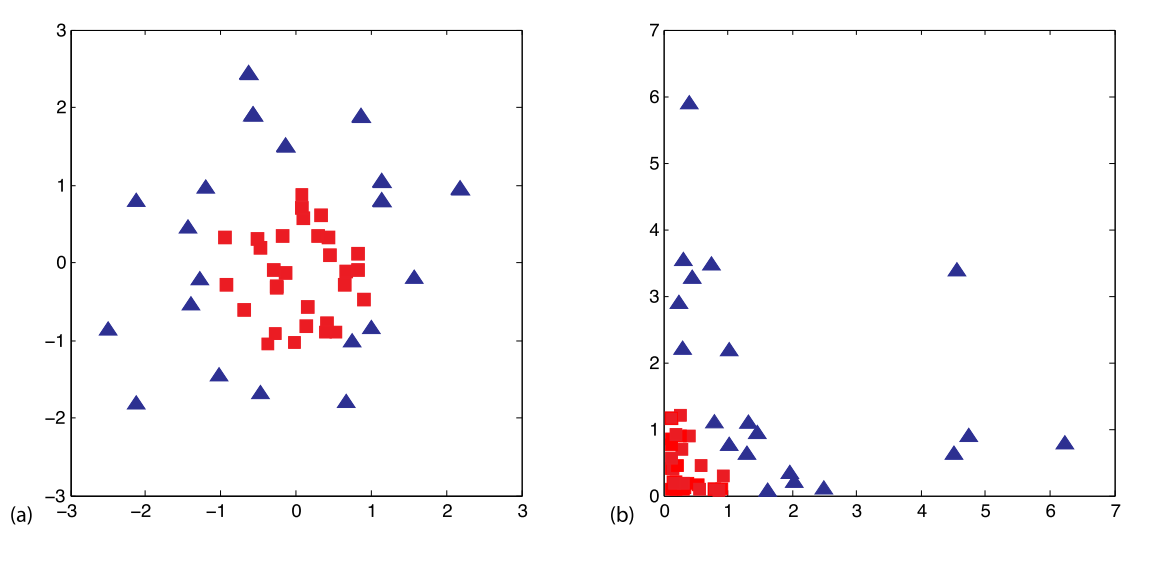
\includegraphics[scale=0.35]{./non-linearly-separable-data.png}
\caption{مثلث‌ها و مربع‌ها دو دسته از داده‌ها را نمایش می‌دهند. در سمت چپ، دو کلاس در فضای اصلی $\mX = \R^2$ قرار دارند و در این فضا خطی‌ جدایی‌پذیر نیستند. در سمت راست، تابع نگاشت $\phi(x) = (x_1^2,x_2^2)$ در فضای $\mH = \R^2$ این داده‌ها را خطی جدایی‌پذیر می‌سازد.}
\label{fig:non-linearly-separable-data}
\end{figure}

ملاحظه می‌کنید که فرم دوگانی SVM تنها از ضرب‌داخلی نقاط $\mx_i,\ldots,\mx_N$ استفاده می‌کند (دستگاه‌های \ارجا{eq:svm-dual-form} و \ارجا{eq:c-svm-dual-form} را ببینید). نکته اینجاست که برای SVM مهم نیست که این ضرب‌داخلی در چه فضایی انجام گرفته است. فضای RKHS $\mH$ را می‌توان با هر RKHS $\mH^\prime$ تعویض کرد. اینجا جایی است که می‌توان از کرنل‌ها به خوبی استفاده کرد: با داشتن کرنل $k: \mX\times \mX \mapsto \R$، می‌توانیم هر $\langle \mx_i,\mx_j \rangle$ را با $k(x_i,x_j)$ جایگزین کنیم. با اینکار، قدرت کرنل‌ها برای نمایش نقاط در فضای با بعد بالاتر را به SVM اضافه می‌کنیم و شاید بتوانیم در آن فضا داده‌ها را به صورت خطی از هم جدا کنیم. بعلاوه از آنجایی که کرنل‌ها را می‌توان روی هر مجموعه‌ای از اشیاء تعریف کرد، پس در واقع SVM هم روی هر مجموعه‌ای از اشیاء قابل استفاده خواهد بود.

اما اگر در SVM از یک تابع اندازه‌گیری شباهت استفاده کنیم که نوعی از ضرب‌داخلی نباشد (متقارن یا نیمه معین مثبت نباشد)، چه اتفاقی خواهد افتاد. پاسخ اینکه توابعی مثل کرنل sigmoid اینچنین هستند و قبلاً در SVM استفاده شده‌اند. ولی در این حالت تضمینی برای محدب بودن مسئله‌ی بهینه‌سازی وجود ندارد و ممکن است دستگاه \ارجا{eq:c-svm-dual-form} اصلاً جواب نداشته باشد\جستار{Burges_1998}.

\subsection{مبانی گراف کرنل‌}\label{sec:graph-kernel-basics}
گراف کرنل‌ها نمونه‌هایی از خانواده‌ی کرنل‌های \متنلاتین{R-convolution} هستند\جستار{Haussler_1999}. \متنلاتین{R-convolution} یک راه کلی برای تعریف کرنل روی اشیاء مرکب است که در آن، یک شیء، تجزیه شده و مقایسه‌ی شباهت روی اجزای اشیاء صورت می‌گیرد. بنابراین هر نوع تجزیه‌ی گراف، به تعریف یک گراف کرنل منجر خواهد شد.

اگر رابطه تجزیه R را داشته باشیم که هر گراف را به تمام زیرگراف‌های ممکن تقسیم کند، کرنل R-convolution وابسته، تمام زیرگراف‌های دو گراف را با هم مقایسه می‌کند. ولی محاسبه این کرنل به اندازه حل مسئله یکریختی سخت خواهد بود\جستار{Gartner_2003}. بنابراین معمولاً کرنل را به مقایسه زیرگراف‌هایی محدود می‌کنند که در زمان خطی محاسبه پذیر باشد.

ذکر این نکته ضروری است که در یادگیری ماشین عبارت \خمیده{گراف کرنل} معمولاً به کرنلی اطلاق می‌شود که رئوس یک گراف بزرگ را با هم مقایسه می‌کند. در این پایان‌نامه، به این نوع کرنل‌ها، کرنل رأسی می‌گوییم و از واژه گراف کرنل برای اشاره به کرنلی استفاده می‌کنیم که گراف‌ها را با یکدیگر مقایسه می‌کند.

گراف کرنل‌های تعریف شده در یادگیری ماشین را می‌توان به سه گروه تقسیم کرد: گراف کرنل‌های مبتنی بر گشت و مسیر، گراف کرنل‌های مبتنی بر زیرگراف‌های کوچک، و گراف کرنل‌های مبتنی بر الگوی زیردرختی. در ادامه به مرور این سه گروه می‌پردازیم.

\subsection{کرنل‌های مبتنی بر گشت و مسیر}\label{sec:random-walk-kernels}
گراف کرنل‌های مبتنی بر گشت و مسیر به ترتیب تعداد گشت‌ها و مسیرهای تصادفی یکسان بین دو گراف را می‌شمارند. الگوریتم استاندارد کرنل گشت تصادفی\جستار{Gartner_2003} روی دو گراف، در $O(n^6)$  قابل محاسبه است. ولی با تبدیل مسئله به حاصلضرب کرونکر\پانوشت{\متنلاتین{Kronecker product}} می‌توان زمان محاسبه را به $O(n^3)$ کاهش داد\جستار{Vishwanathan_2010}. هرچند که این کاهش در زمان محاسبه قابل توجه است، اما پیچیدگی $O(n^3)$ هنوز بسیار بالاست. علاوه بر این، کرنل‌های مبتنی بر گشت دو مشکل دیگر هم دارند: \خمیده{رفت و برگشت}\پانوشت{tottering}\جستار{Mahe_2004} و \خمیده{هالتینگ}\پانوشت{halting}\جستار{Borgwardt_2007}.

مشکل رفت و برگشت از این حقیقت سرچشمه می‌گیرد که طبق تعریف، یک گشت اجازه تکرار رئوس و یال‌ها را دارد. در نتیجه، یک یال مشترک در دو گراف، می‌تواند به تعداد نامتناهی روی مقدار کرنل تأثیرگذار باشد. برای حلقه‌ها و مسیرهای مشترک بین دو گراف هم این وضعیت وجود دارد. بنابراین مقدار کرنل برای دو گراف که شباهت ساختاری به هم ندارند می‌تواند بی‌جهت بزرگ شود.

و اما مشکل هالتینگ. همانطور که دیدیم کرنل گشت تصادفی، تعداد \خمیده{تمام} گشت‌های مشترک بین دو گراف را می‌شمارد. از طرفی، تعداد گشت‌های حداقل به طول یک در یک گراف، ناشماراست. بنابراین معمولاً یک فاکتور کاهنده $\lambda$ روی طول گشت در نظر می‌گیرند که وزن گشت‌های بلند را کم می‌کند. هرچند که با اینکار مقایسه دو گراف با در نظر گرفتن تمام گشت‌ها ممکن می‌شود ولی گشت‌های کوچک بر مقدار کرنل چیره می‌شوند. به این مشکل، \خمیده{هالتینگ} می‌گویند.

کرنل کوتاهترین مسیر، طول کوتاهترین مسیر بین هر دو رأس مشترک بین دو گراف (که با برچسب مشخص می‌شوند) را مقایسه می‌کند\جستار{Borgwardt_2005}. پیچیدگی محاسباتی این کرنل برابر $O(n^4)$ است. به وسیله این کرنل، گراف کرنل‌هایی کارا مختص مولکول‌های کوچک با میانگین درجه بین دو تا سه تعریف شده‌اند که مسیرهای برچسب‌دار به طول $p$ را می‌شمارند\جستار{Ralaivola_2005}. این مسیر‌ها توسط الگوریتم جستجوی عمق-اول برای هر رأس محاسبه می‌شوند.

\subsection{کرنل‌های مبتنی بر زیرگراف‌های کوچک}\label{sec:subgraph-kernels}
این گروه، شامل کرنل‌های مبتنی بر شمارش زیرگراف‌های کوچک یا به اصطلاح \خمیده{گرافلت‌ها}\پانوشت{graphlets} است. در این روش، هر گراف به شکل برداری از تعدادِ زیرگراف‌های سه تا پنج رأسی نمایش داده می‌شود. محاسبه‌ی مقدار کرنل برای دو گراف به این صورت انجام می‌شود که ابتدا بردار گرافلت برای آن دو محاسبه می‌شود، سپس با ضرب داخلی این دو بردار، میزان شباهت دو گراف بدست می‌آید\جستار{Shervashidze_2009}. بهترین الگوریتم برای محاسبه بردار گرافلت، دارای پیچیدگی $O(nd^{k-1})$ است که در آن $k = \lbrace{3,4,5}\rbrace$ اندازه گرافلت و $d$ بزرگترین درجه گراف است. در فصل \ارجا{chap:gaussian-graphlet-kernel} راجع به این کرنل‌ها به تفصیل سخن خواهیم گفت و مشکلات آن‌ را بررسی خواهیم کرد.
کرنل‌های الگوهای دوری\پانوشت{\متنلاتین{cyclic pattern kernels}}\جستار{Horvath_2004}، تعداد حلقه‌های مشترک بین دو گراف را می‌شمارند. محاسبه این کرنل به طور کلی مسئله‌ای \متنلاتین{NP-hard} است و تنها برای برخی گراف‌هاست که می‌توان مقدار کرنل را به صورت بهینه محاسبه کرد. کرنل دیگری که در این گروه قرار می‌گیرد، بر اساس تجزیه گراف به زیرگراف‌های همسایگی به شعاع $r$ و به فاصله $d$ تعریف می‌شود\جستار{Costa_2010}. میزان شباهت دو گراف برابر تعداد زیرگراف‌های یکریخت بین آن‌ها خواهد بود. این کرنل برای گراف‌های کوچک و همچنین $r$ و $d$ بسیار کوچک پیچیدگی تقریباً $O(n)$ خواهد داشت ولی با افزایش $d$ و $r$ مسئله به تست یکریختی دو گراف نزدیک خواهد شد.

\subsection{کرنل‌های مبتنی بر الگوهای زیردرختی}
اولین کرنل از این گروه در سال ۲۰۰۳ تعریف شد\جستار{Ramon_2003}. در این کرنل، برای محاسبه میزان شباهت دو گراف $G$ و $G^\prime$، برای هر جفت رأس $v \in G$ و $v^\prime \in G^\prime$، تمام زیرساختارهای یکریخت از دو درخت ریشه گرفته از $v$ و $v^\prime$ شمرده می‌شوند. محاسبه‌ی این کرنل کار دشواری است: برای مجموعه $N$ تایی از گراف‌ها، پیچیدگی محاسباتی برابر $O(N^2n^2h4^d)$ خواهد بود که $n$ تعداد رئوس گراف، $h$ ارتفاع بزرگترین زیردرخت در نظر گرفته شده و $d$ حداکثر درجه در گراف‌های این مجموعه است. کرنل‌های دیگری بر مبنای این کرنل در کاربردهایی نظیر شیمی محاسباتی\جستار{Mahe_2009} و پردازش تصویر\جستار{Bach_2008} تعریف شده‌اند که برای گراف‌های کوچک مناسب هستند ولی بازهم رشد پیچیدگی آن‌ها تابعی نمایی از اندازه گراف است.

\subsection{گراف‌کرنل‌های ویسفلر-لیمن}\label{sec:weisfeiler-lehman-kernels}
 خانواده‌ی کرنل‌های ویسفلر-لیمن\پانوشت{\متنلاتین{Weisfeiler-Lehman}}\جستار{Shervashidze_2011} بر اساس تست همریختی با همین نام پایه‌ریزی شده‌اند. ایده اصلی در این کرنل‌ها برچسب‌گذاری دوباره رئوس است. الگوریتم به صورت مرحله‌ای اجرا می‌شود. تعداد مراحل با پارامتر ارتفاع $h$ کنترل می‌گردد. در هر مرحله از اجرای الگوریتم، برای هر رأس $v$ از گراف $G$، زیرگرافی از $G$ در نظر گرفته می‌شود که شعاع آن از رأس $v$ حداکثر $h$ باشد. سپس به برچسب $v$، مجموعه‌ی مرتبی از برچسب‌های رئوس این زیرگراف افزوده می‌شود و این برچسب‌ها در قالب یک برچسب جدید فشرده می‌شوند. حال می‌توان از هر کرنل $k$ که روی گراف‌های برچسب‌دار تعریف شده باشد استفاده کرد و شباهت دو گراف دوباره برچسب‌دهی شده را اندازه گرفت. بر این اساس، سه کرنل ویسفلر-لیمن زیردرختی، یالی و کوچکترین مسیر تعریف شده‌اند\جستار{Shervashidze_2011}. پیچیدگی محاسبه ویسفلر-لیمن زیردرختی برای مجموعه $N$ گراف برابر  $O(Nhm+N^2hn)$ است که $h$ پارامتر ارتفاع و $n$ و $m$ به ترتیب تعداد رئوس و یال‌های بزرگترین گراف این مجموعه هستند. با این وجود این کرنل مانند کرنل گشت تصادفی، از مشکل رفت و برگشت رنج می‌برد\جستار{Bai_2014}. کرنل‌های ویسفلر-لیمن یالی و کوچکترین مسیر علاوه بر زمان اجرای زیاد، نیاز به حافظه زیادی دارند که استفاده از آن‌ها را برای مجموعه گراف‌های بزرگ غیر ممکن می‌کند (رجوع شود به بخش ۳.۳.۱ و ۳.۴.۱ \جستار{Shervashidze_2011}).
 
\section{جمع‌بندی}
در این بخش تئوری‌های مورد نیاز برای فصول آینده را مرور کردیم و مهمترین گراف کرنل‌ها در یادگیری ماشین را معرفی نمودیم. همانطور که در بخش‌ \ارجا{sec:graph-kernels-review} دیدیم، هر کرنل نیمه معین مثبت روی گراف‌ها به شکل $k(G,G^\prime) = \lbrace{\phi(G),\phi(G^\prime)}\rbrace$ تعریف می‌شود که $\phi(G)$ نمایش ویژگی $G$ در فضای هیلبرت بازتولید کرنل است: انتخاب $k$ (بطور معادل، انتخاب $\phi$) پاسخی برای هر دو مسئله‌ی مقایسه و نمایش گراف است. همچنین، دیدیم که گراف کرنل‌ها به ما امکان می‌دهند طیف وسیعی از تکنیک‌های یادگیری ماشین را روی ساختارهای پیچیده در قالب گراف پیاده‌سازی کنیم.

با توجه به توضیحات بخش \ارجا{sec:graph-kernel-basics}، گراف کرنل‌های موجود دارای مشکلاتی هستند که مهمترین آن‌ها پیچیدگی زمانی بالاست. در مورد گراف کرنل ویسفلر-لیمن زیردرختی که زمان اجرای خوبی دارد، مشکل رفت و برگشت از دقت آن در مقایسه گراف‌ها را می‌کاهد.

در فصل بعد، گرافلت کرنل‌ها را با دقت بیشتری بررسی می‌کنیم و سعی می‌کنیم با محاسبه بهینه تعداد گرافلت‌ها، مشکل پیچیدگی زمانی این نوع از کرنل‌ها را برطرف کنیم. سپس با محاسبه فاصله بین بردارهای گرافلت (متناظر با گراف‌های تحت بررسی) در فضای بالاتر، دقت این کرنل را افزایش دهیم.
